% Pro kompilaci po částech (viz projekt.tex), nutno odkomentovat a upravit
%\documentclass[../projekt.tex]{subfiles}
%\begin{document}

\chapter{Úvod}

\chapter{Vizualizácia dát z~mobilných mapovacích systémov}

[stručný popis, aké dáta produkujú m. m. s.]

\section{Dierkový model kamery -- teoretický základ zobrazenia}

[...]

\section{Existujúce možnosti zobrazenia dát z~mobilných mapovacích systémov}

[popis základných knižníc aj programov, ako napr. CloudCompare]

\subsection{Riešenia dostupné v~jazyku Python}

\subsubsection{Framework deck.gl a jeho nadstavba Pydeck}
\label{sec:deck_gl}

Javascriptový framework deck.gl je určený na zobrazovanie dát najmä na mapových podkladoch. Vyznačuje sa vysokou presnosťou a výkonnosťou. Pre akceleráciu využíva rozhrania WebGPU a WebGL2 \cite{deck.gl_documentation}.

Vizualizácia dát v~deck.gl sa skladá z~dvoch základných častí:
\begin{itemize}
    \item Vrstvy (\texttt{Layers}). Do vrstiev sa ukladajú zobrazované dáta. Framework deck.gl ponúka vyše 30 preddefinovaných typov vrstiev. Pre túto prácu je významná najmä vrstva \texttt{PointCloudLayer}, ktorá je určená na zobrazenie mračna bodov, a vrstva \texttt{LineLayer}, ktorá je určená na zobrazenie čiar.
    \item Pohľad (\texttt{View}). Definuje vlastnosti kamery, napríklad zorné pole a prednú a zadnú orezávaciu rovinu (\emph{near plane} a \emph{far plane}).
    Časť \texttt{ViewState} určuje polohu a smer pohľadu kamery. Typ pohľadu definuje spôsob interakcie vizualizácie s~používateľom, napríklad pre zobrazenie trate z~pohľadu strojvedúceho je ideálny typ \texttt{FirstPersonView}.
\end{itemize}

Napriek tomu, že je framework deck.gl primárne určený pre použitie v~Javascripte, je možné ho použiť aj v~jazyku Python, a to pomocou knižnice \textbf{Pydeck}. Tá je pomerne jednoduchá a podstatou jej činnosti je, že prevedie kód napísaný v~jazyku Python do formátu JSON. Framework deck.gl má totiž modul @deck.gl/json, ktorý prijíma reprezentáciu vizualizácie vo formáte JSON a transformuje ju do javascriptového kódu (na definície funkcií a deck.gl objektov)\footnote{Ukážka rozhrania modulu @deck.gl/json je na \url{https://deck.gl/playground}.}.

Knižnica Pydeck je dobrým prostriedkom na vytvorenie jednoduchých vizualizácií, s~ktorými môže používateľ interagovať pohybmi myši. Jej možnosti sú však oproti pôvodnému frameworku deck.gl veľmi obmedzené. Nie je však vhodná na vytváranie zložitejších animácií s~veľkým množstvom dát, pretože sa aj po tej najmenšej zmene musia dáta a definícia vizualizácie nanovo prevádzať do formátu JSON a následne na javascriptový kód (obrázok \ref{fig:pydeck_dashdeck_schema}), čo je veľmi časovo náročné.

\begin{figure}[h]
    \centering
    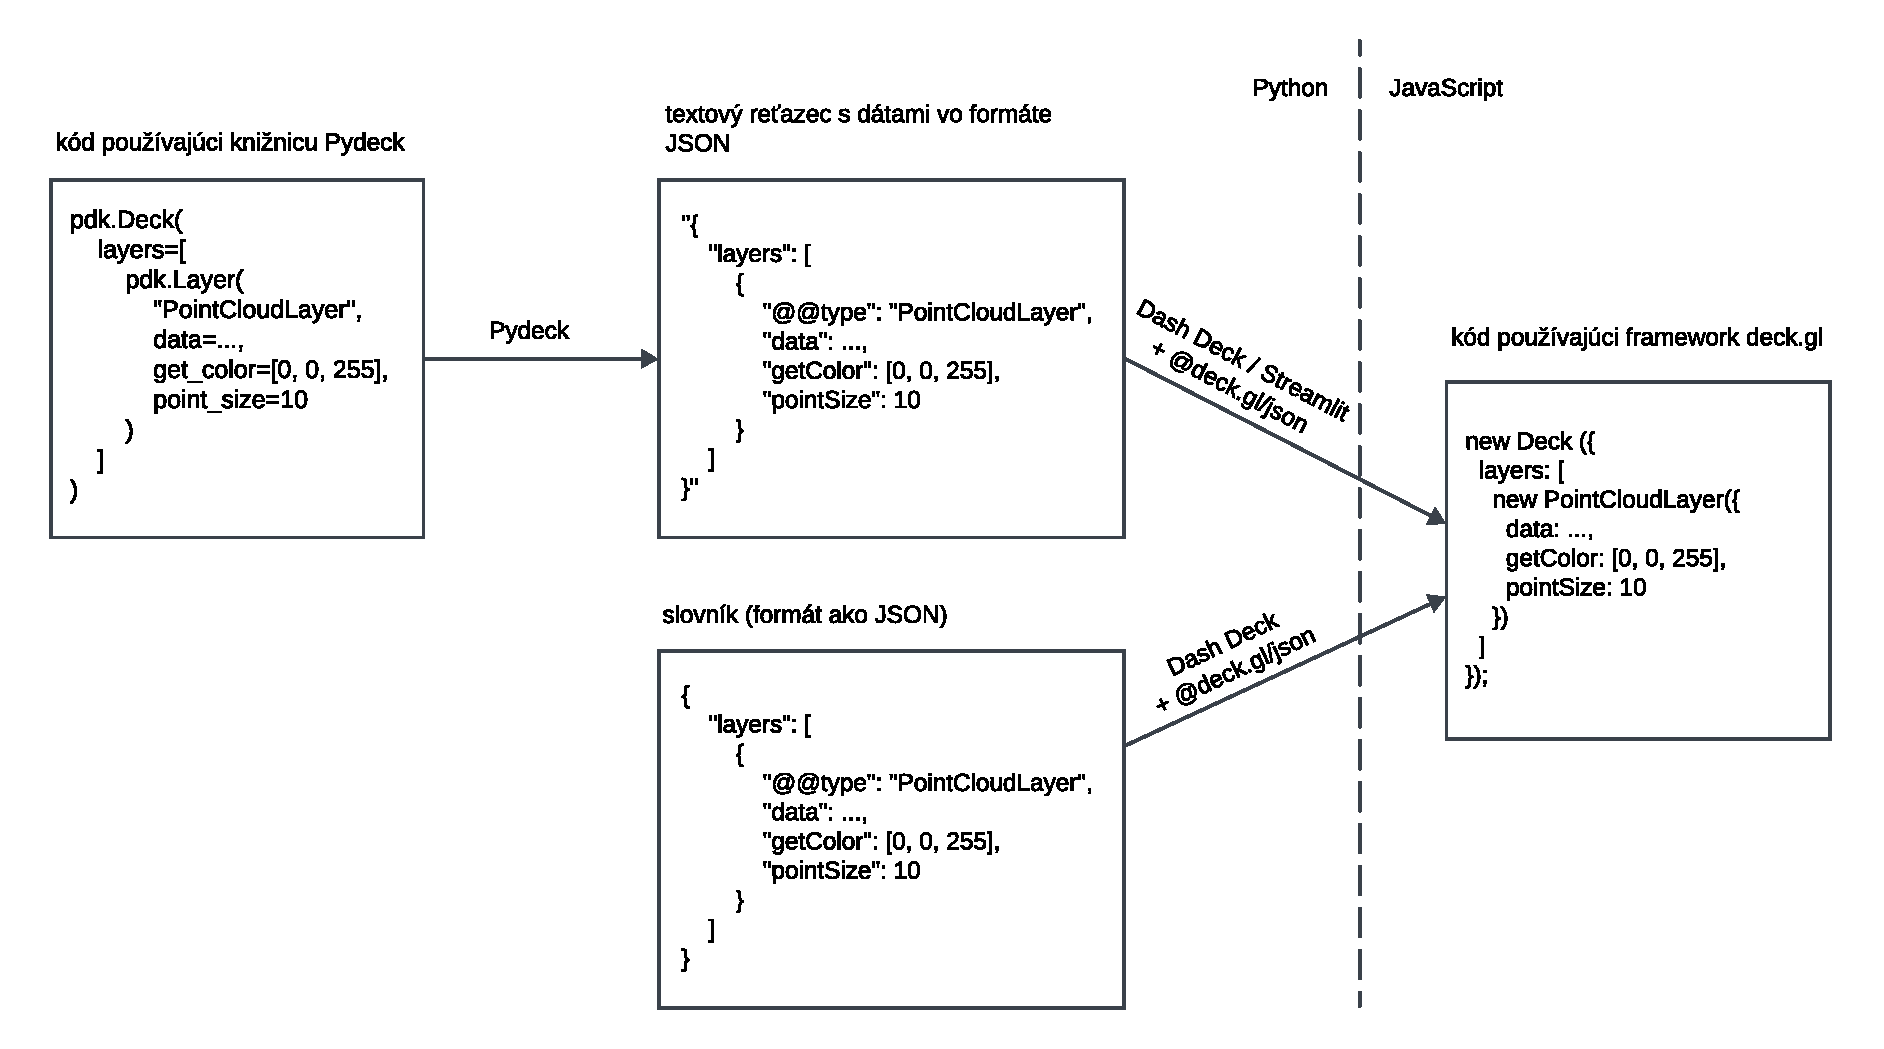
\includegraphics[width=1\linewidth]{text_prace/obrazky-figures/pydeck_dashdeck_transformacie.pdf}
    \caption{Schéma vzťahov medzi technológiami Pydeck, Dash Deck a deck.gl.}
    \label{fig:pydeck_dashdeck_schema}
\end{figure}

\section{Frameworky pre tvorbu interaktívnej webovej aplikácie v~jazyku Python}

\subsubsection{Porovnanie frameworkov Streamlit a Dash}

Streamlit a Dash sú frameworky, ktoré majú rovnaké zameranie: oba slúžia na tvorbu webových aplikácií pre prácu s~dátami (\emph{data apps}) v~jazyku Python. Dash je oproti Streamlitu na nižšej úrovni abstrakcie, pretože sám o~sebe nemá žiaden vizuálny štýl a mnohé jeho komponenty sa priamo mapujú na HTML elementy, napríklad \texttt{dash.html.Div} a \texttt{dash.html.H1} \cite{streamlit_documentation}\cite{dash_documentation}.

Oba frameworky majú podporu pre Pydeck, u~Streamlitu je priamo k~dispozícii element \texttt{st.pydeck\_chart} a k~Dashu má na tento účel vytvorenú prídavnú knižnicu \textbf{Dash Deck}. Ukázalo sa však, že \texttt{st.pydeck\_chart} podporuje iba pohľad \texttt{MapView}, ktorý je určený na zobrazenie dát na mape a nedá sa použiť na perspektívne zobrazenie bodov v~trojrozmernom priestore.

Dash Deck má navyše tú výhodu, že umožňuje vynechať Pydeck a definovať zobrazenie pomocou slovníkov so štruktúrou zodpovedajúcou tej, ktorú vyžaduje modul @deck.gl/json, čo je znázornené na obrázku \ref{fig:pydeck_dashdeck_schema}. To trochu zefektívni vykonávanie zmien vo vizualizácii, keďže taká reprezentácia umožní jednoduchšie vykonávanie úprav.

\subsubsection{Popis frameworku Dash}

[...]

\chapter{Návrh aplikácie pre vizualizáciu dát z~železničného mobilného mapovacieho systému}

Cieľom tejto práce je vytvoriť používateľskú aplikáciu. Výsledná aplikácia by mala byť webová, aby ju bolo možné spustiť jednoducho pomocou webového prehliadača. Mala by spĺňať nasledujúce body:

\begin{itemize}
    \item Zobrazenie dát z~mobilného mapovacieho systému. Tieto dáta sú tvorené mračnom bodov, kamerovým záznamom, vektorovými dátami a údajmi o~pohybe vlaku a mali by byť zobrazené z~pohľadu strojvedúceho vlaku.
    \item Umožniť používateľovi vybrať si konkrétnu pozíciu vlaku aj prehrať si animáciu pohybu vlaku.
    \item Umožniť používateľovi nahrať súbory s~dátami na zobrazenie: súbor s~mračnom bodov, video z~kamery na čele vlaku, súbor s~vektorovými dátami, textové súbory s~údajmi o~pohybe vlaku - pole translácií a pole rotácií.
    \item Poskytnúť používateľovi možnosti prispôsobenia zobrazenia, ako napríklad zmeny viditeľnosti jednotlivých vrstiev (mračno bodov, vektorové dáta, kamerový záznam) a základné nastavenia zobrazenia mračna bodov (rôzne farebné škály podľa intenzity, veľkosť a priehľadnosť bodov, zobrazenie bodov len do určitej vzdialenosti) aj vektorových dát (farba a hrúbka čiar). Užitočná by bola aj možnosť doladiť parametre zobrazovania mračna bodov a vektorových dát (posun aj otočenie kamery doprava/doľava, nahor/nadol, ohnisková vzdialenosť), aby bolo možné toto zobrazenie prispôsobiť záznamu z~kamery. Kamera totiž môže byť na vlaku rôzne umiestnená a údaje z~nej môžu byť oproti údajom z~mračna bodov posunuté.
    \item Zobrazovať prejazdný profil vlaku v~istej vzdialenosti pred vlakom a umožnovať prehrať animáciu jeho pohybu (podľa vektorových údajoch o~koľajniciach).
    \item Detekovať prekážky na trati.
    \item Umožňovať kolorizáciu mračna bodov podľa kamerového záznamu.
\end{itemize}

\section{Návrh používateľského rozhrania}

[návrh vrátane popisu zvolených farebných škál]

\chapter{Implementácia navrhnutej aplikácie}

Prvou fázou implementácie bolo napísanie skriptu v~jazyku Python, ktorý vykresľoval mračno bodov bez použitia špeciálnych knižníc či frameworkov. K~dispozícii pritom bola jedna sada ukážkových dát, ktorá sa skladala z~mračna bodov, kalibračnej matice a postupnosti translácií a rotácií, ktoré predstavovali pohyb vlaku po trati. Mračno bodov obsahovalo 201~880 bodov s~intenzitou od 0 do 42 a bolo definovaných 500 polôh vlaku. K~tomu boli dodané obrázky, ktoré ukazovali, ako by mal vyzerať výsledok zobrazenia (obrázok \ref{fig:referencny-obrazok}).

\begin{figure}[h]
    \centering
    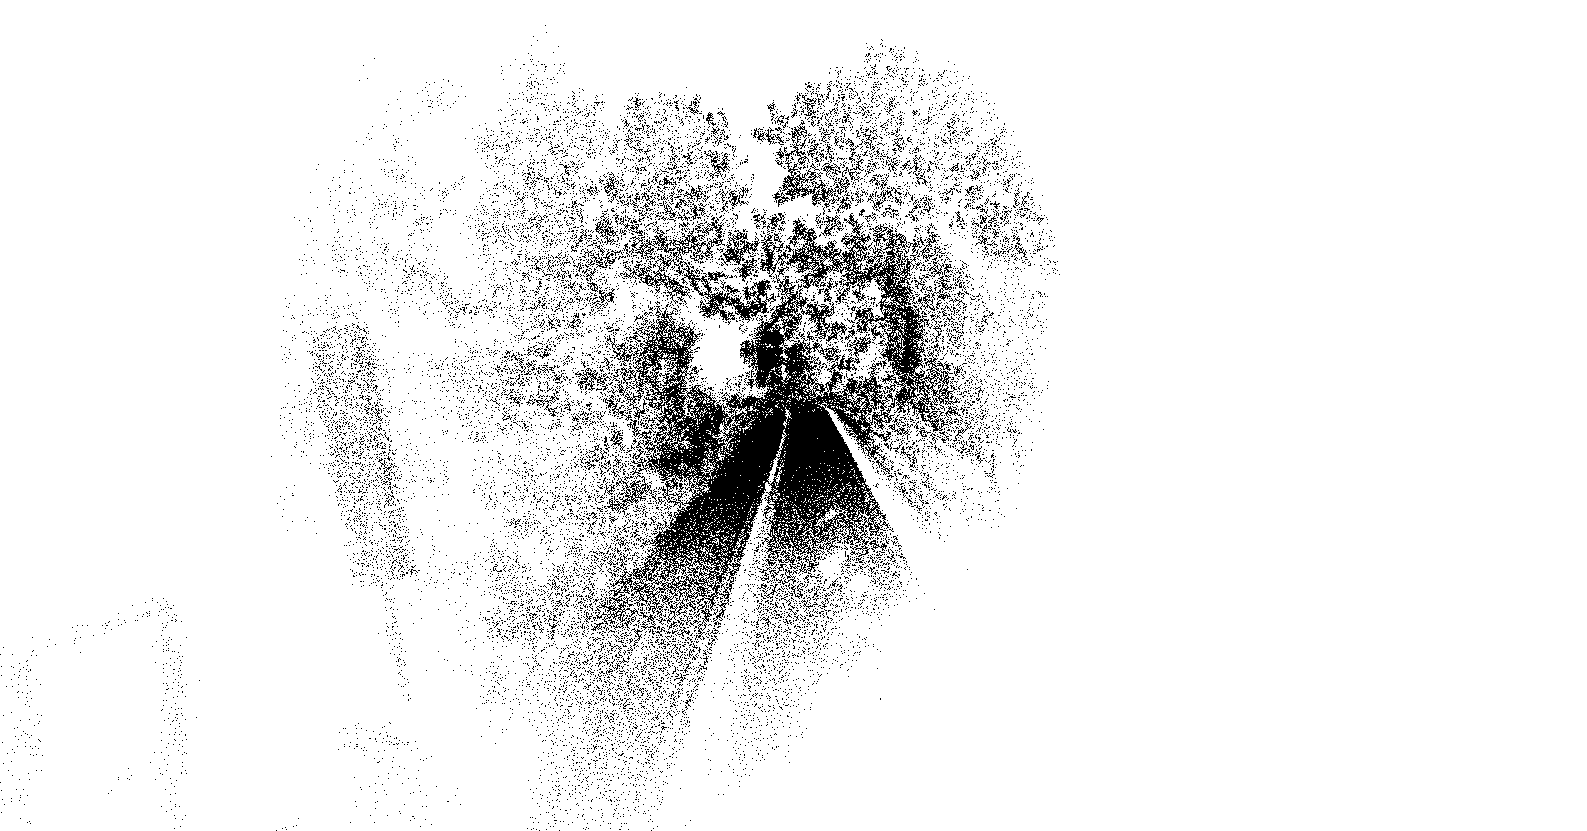
\includegraphics[width=0.95\linewidth]{obrazky-figures/referencny_obrazok.png}
    \caption{Referenčný obrázok, ktorý bol dodaný na začiatku práce spolu s~mračnom bodov a údajmi o~pohybe kamery v~ňom. Obrázok je tu pre lepšiu viditeľnosť s~invertovanými farbami a zväčšeným kontrastom.}
    \label{fig:referencny-obrazok}
\end{figure}

Cieľom tejto prvotnej fázy bolo najmä oboznámenie sa s~dátami a základnými princípmi vykresľovania bodov. Výsledky, ktoré sa nakoniec podarilo dosiahnuť, boli podobné referenčným obrázkom, aj keď nie úplne identické. Ukázalo sa, že údaje o~pohybe kamery majú iný súradnicový systém ako mračno bodov (líšilo sa poradie ôs) a že je potrebné pridať isté posunutie a otočenie, aby sa výsledky podobali referenčným obrázkom (posunutie kamery do stredu vlaku, podľa dodaných dát bola naľavo od stredu).

Ďalej už nasledovala práca s~existujúcimi knižnicami a frameworkami v~jazyku Python. Prvotným plánom bolo použiť knižnicu Pydeck (pre vizualizáciu dát) s~frameworkom Streamlit (pre tvorbu GUI). Pydeck bol zvolený preto, že je nadstavbou nad javascriptovým frameworkom deck.gl, ktorý na vykresľovanie dát využíva grafickú kartu a má dobrú výkonnosť. Ukázalo sa však, že Streamlit nepodporuje Pydeck v~plnej miere, a teda sa nedá využiť. Preto bol namiesto Streamlitu použitý framework Dash, ktorý už mal podporu pre Pydeck dostatočnú.

Pomocou tohto frameworku bola vytvorená jednoduchá webová aplikácia zobrazujúca ukážkové dáta a umožňujúca základné nastavenia vzhľadu. Do tejto aplikácie bolo zahrnuté aj zobrazovanie kamerového záznamu, pre tento účel bolo provizórne použité video z~prejazdu tej istej trate natočené v~roku 2012. Pri tom sa zistilo, že vykresľovanie dát pomocou kombinácie knižníc Pydeck a Dash Deck tak, ako je to vo vzorových príkladoch v~dokumentácii knižnice Dash Deck, je značne neefektívne. Jedno vykreslenie mračna bodov zaberalo zhruba 3 sekundy, čo bolo spôsobené transformáciami medzi rôznymi formátmi, ako to bolo popísané v~sekcii \ref{sec:deck_gl}.

Tento čas sa podarilo významne zredukovať použitím knižnice Dash Deck bez knižnice Pydeck. Výsledok však stále nebol dosť dobrý na to, aby mohla hladko bežať animácia pohybu vlaku, a ani napriek rôznym pokusom sa ho už nepodarilo v~rámci tejto kombinácie technológií vo významnejšej miere vylepšiť. Čas vykreslenia mračna bodov bol pritom úmerný počtu bodov a príčina neefektivity bola v~spôsobe implementácie knižnice Dash Deck. Na výkonnosť malo navyše vplyv aj zobrazovanie videa. Bolo preto rozhodnuté optimalizovať vykresľovanie dát vynechaním knižnice Dash Deck a použitím frameworku deck.gl priamo z~jazyka Javascript.

\section{Optimalizácia vykresľovania mračna bodov priamym použitím jazyka JavaScript}

Pythonový framework Dash interne používa na vytváranie používateľského rozhrania JavaScript, konkrétne framework React \cite{dash_documentation}. Jeho tvorcovia rátali s~tým, že vývojári, ktorí ho budú používať, budú niekedy chcieť priamo použiť javascriptový kód. Preto to tento framework umožňuje viacerými spôsobmi:

\begin{itemize}
    \item Klientske callbacky. Podobajú sa tým štandardným, ale na rozdiel od nich bežia iba na klientovi a píšu sa v~jazyku JavaScript. Štandardné callbacky bežia na serveri a píšu sa v~Pythone.
    \item Skripty v~jazyku JavaScript, ktoré je možné pripojiť k~generovanej HTML stránke. Spustia sa automaticky pri otvorení stránky v~prehliadači.
    \item Vytváranie vlastných komponentov používateľského rozhrania pomocou frameworku React.
\end{itemize}

V~tejto práci bola pre jednoduchosť využitá prvá a druhá možnosť. Bol napísaný skript \texttt{visualisation.js}, v~ktorom sú definované funkcie pre zobrazenie a zmeny zobrazenia dát pomocou deck.gl. Odkazy na tieto funkcie sú potom priradené do objektu \texttt{window}, aby bolo možné volať ich z~klientskych callbackov. Tento objekt teda tvorí rozhranie skriptu \texttt{visualisation.js}, ktoré je využívané zvyškom kódu aplikácie.

Pre správne pripojenie zdrojových kódov frameworku deck.gl k~javascriptovému kódu tak, aby mohol fungovať v~rámci aplikácie napísanej vo frameworku Dash, je nutné použiť bundler. V~rámci tejto práce bol použitý bundler Webpack. Výstupnému skriptu je potrebné nastaviť príponu \texttt{.mjs}, aby ho Dash spustil ako modul.

Výkonnosť vykresľovania mračna bodov pred a po optimalizácii je vzhľadom na riadenie animácie pomocou komponentu \texttt{Interval} pomerne ťažké určiť. Ten má síce podľa dokumentácie zabezpečovať periodické volanie funkcií, ale v~praxi sa ukázalo, že jeho presnosť nie je veľká a navyše animáciu spomaľuje, pretože funguje na základe komunikácie medzi klientom a serverom. Preto by bolo vhodné ho niečím nahradiť, napríklad riadením animácie v~Javascripte iba na klientskej strane.


\begin{table}[h]
    \centering
    \begin{tabular}{m{10em}|m{13em}|m{12em}}
        {\RaggedRight Nastavenie parametra \texttt{interval} [ms]} &  {\RaggedRight Čas, za ktorý prebehla celá animácia (500 snímok) [s]} & {\RaggedRight Priemerný čas vykreslenia jedného snímku [ms]} \\ \hline
         &  &  \\
         &  &  \\
    \end{tabular}
    \caption{Výkonnosť vykresľovania mračna bodov obsahujúceho 201~880 bodov pred optimalizáciou, teda iba pomocou kódu v~jazyku Python. Použité technológie: Python, Dash, Dash Deck.}
    \label{tab:js_optimalizacia}
\end{table}

\begin{table}[h]
    \centering
    \begin{tabular}{m{10em}|m{13em}|m{12em}}
        {\RaggedRight Nastavenie parametra \texttt{interval} [ms]} &  {\RaggedRight Čas, za ktorý prebehla celá animácia (500 snímok) [s]} & {\RaggedRight Priemerný čas vykreslenia jedného snímku [ms]} \\ \hline
         &  &  \\
         &  &  \\
    \end{tabular}
    \caption{Výkonnosť vykresľovania mračna bodov obsahujúceho 201~880 bodov po optimalizácii, teda iba pomocou vloženia kódu v~jazyku Javascript. Použité technológie: Python, Dash, Javascript, deck.gl.}
\end{table}


\section{Experimenty a vyhodnotenie výsledkov}

\chapter{Záver}


%===============================================================================

% Pro kompilaci po částech (viz projekt.tex) nutno odkomentovat
%\end{document}

